\documentclass[paper=letter,11pt]{scrartcl}

\KOMAoptions{headinclude=true, footinclude=false}
\KOMAoptions{DIV=14, BCOR=5mm}
\KOMAoptions{numbers=noendperiod}
\KOMAoptions{parskip=half}
\addtokomafont{disposition}{\rmfamily}
\addtokomafont{part}{\LARGE}
\addtokomafont{descriptionlabel}{\rmfamily}
%\setkomafont{pageheadfoot}{\normalsize\sffamily}
\setkomafont{pagehead}{\normalsize\rmfamily}
%\setkomafont{publishers}{\normalsize\rmfamily}
\setkomafont{caption}{\normalfont\small}
\setcapindent{0pt}
\deffootnote[1em]{1em}{1em}{\textsuperscript{\thefootnotemark}\ }


\usepackage{amsmath}
\usepackage[varg]{txfonts}
\usepackage[T1]{fontenc}
\usepackage{graphicx}
\usepackage{xcolor}
\usepackage[american]{babel}
% hyperref is needed in many places, so include it here
\usepackage{hyperref}

\usepackage{xspace}
\usepackage{multirow}
\usepackage{float}


\usepackage{braket}
\usepackage{bbm}
\usepackage{relsize}
\usepackage{tcolorbox}

\def\ketY{\ensuremath{\ket {\Psi}}}
\def\iGeV{\ensuremath{\textrm{GeV}^{-1}}}
%\def\mp{\ensuremath{m_{\textrm{proton}}}}
\def\rp{\ensuremath{r_{\textrm{proton}}}}
\def\me{\ensuremath{m_{\textrm{electron}}}}
\def\aG{\ensuremath{\alpha_G}}
\def\rAtom{\ensuremath{r_{\textrm{atom}}}}
\def\rNucl{\ensuremath{r_{\textrm{nucleus}}}}
\def\GN{\ensuremath{\textrm{G}_\textrm{N}}}
\def\ketX{\ensuremath{\ket{\vec{x}}}}
\def\ve{\ensuremath{\vec{\epsilon}}}


\def\ABCDMatrix{\ensuremath{\begin{pmatrix} A &  B  \\ C  & D \end{pmatrix}}}
\def\xyprime{\ensuremath{\begin{pmatrix} x' \\ y' \end{pmatrix}}}
\def\xyprimeT{\ensuremath{\begin{pmatrix} x' &  y' \end{pmatrix}}}
\def\xy{\ensuremath{\begin{pmatrix} x \\ y \end{pmatrix}}}
\def\xyT{\ensuremath{\begin{pmatrix} x & y \end{pmatrix}}}

\def\IMatrix{\ensuremath{\begin{pmatrix} 0 &  1  \\ -1  & 0 \end{pmatrix}}}
\def\IBoostMatrix{\ensuremath{\begin{pmatrix} 0 &  1  \\ 1  & 0 \end{pmatrix}}}
\def\JThree{\ensuremath{\begin{pmatrix}    0 & -i & 0  \\ i & 0  & 0 \\ 0 & 0 & 0 \end{pmatrix}}} 
\def\JTwo{\ensuremath{\begin{bmatrix}    0 & 0 & -i  \\ 0 & 0  & 0 \\ i & 0 & 0 \end{bmatrix}}}
\def\JOne{\ensuremath{\begin{bmatrix}    0 & 0 & 0  \\ 0 & 0  & -i \\ 0 & i & 0 \end{bmatrix}}}
\def\etamn{\ensuremath{\eta_{\mu\nu}}}
\def\Lmn{\ensuremath{\Lambda^\mu_\nu}}
\def\dmn{\ensuremath{\delta^\mu_\nu}}
\def\wmn{\ensuremath{\omega^\mu_\nu}}
\def\be{\begin{equation*}}
\def\ee{\end{equation*}}
\def\bea{\begin{eqnarray*}}
\def\eea{\end{eqnarray*}}
\def\bi{\begin{itemize}}
\def\ei{\end{itemize}}
\def\fmn{\ensuremath{F_{\mu\nu}}}
\def\fMN{\ensuremath{F^{\mu\nu}}}
\def\bc{\begin{center}}
\def\ec{\end{center}}
\def\nus{$\nu$s}

\def\adagger{\ensuremath{a_{p\sigma}^\dagger}}
\def\lineacross{\noindent\rule{\textwidth}{1pt}}

\newcommand{\multiline}[1] {
\begin{tabular} {|l}
#1
\end{tabular}
}

\newcommand{\multilineNoLine}[1] {
\begin{tabular} {l}
#1
\end{tabular}
}



\newcommand{\lineTwo}[2] {
\begin{tabular} {|l}
#1 \\
#2
\end{tabular}
}

\newcommand{\rmt}[1] {
\textrm{#1}
}


%
% Units
%
\def\m{\ensuremath{\rmt{m}}}
\def\GeV{\ensuremath{\rmt{GeV}}}
\def\pt{\ensuremath{p_\rmt{T}}}


\def\parity{\ensuremath{\mathcal{P}}}

\usepackage{cancel}
\usepackage{ mathrsfs }
\def\bigL{\ensuremath{\mathscr{L}}}

\usepackage{ dsfont }



\usepackage{fancyhdr}
\fancyhf{}


\lhead{\Large 33-444} % \hfill Introduction to Particle Physics \hfill Spring 2022}
\chead{\Large Introduction to Particle Physics} % \hfill Spring 2022}
\rhead{\Large Spring 2022} % \hfill Introduction to Particle Physics \hfill Spring 2022}
\begin{document}
\thispagestyle{fancy}





%\begin{tabular}{c}
%{\large 33-444 \hfill Intro To Particle \hfill Spring 2022\\}
%\hline 
%\end{tabular}

\begin{center}
{\huge \textbf{Homework Set \#4}}
\large

{\textbf{ Solutions  }} 
\end{center}

{\large
\textbf{1) Find the generators of the ``Little Group'' for Massive particles \hfill \textit{(5 points)}}

The little group equation is:
\be
W\cdot k = k \Rightarrow \omega \cdot k = 0
\ee

where
\be
\omega_{\mu\nu} = \begin{bmatrix} 0 & a & b & c \\ -a & 0 & A & B \\ -b & -A & 0 & C \\ -c & -B & -C & 0 \end{bmatrix}
\ee


For a massive particle we can take k to be k = (m,0,0,0).

So $\omega \cdot k = (0,-ma,-mb,-mc) $. So the little group generators for massive particles are 
\be
\omega_{\mu\nu} = \begin{bmatrix} 0 & 0 & 0 & 0 \\ 0 & 0 & A & B \\ 0 & -A & 0 & C \\ 0 & -B & -C & 0 \end{bmatrix}
\ee
which are the rotation matrices.

\vspace*{0.25in}

\textbf{2) Heisenberg Equation of Motion \hfill \textit{(5 points)}}
\begin{itemize}
\item[a)] { 

\begin{eqnarray*}
\frac{dA(t)_H}{dt} =& \frac{d}{dt}\left( e^{iHt} A_s e^{-iHt}\right)\\
=& iH \left(e^{iHt} A_s e^{-iHt}\right) - i \left(e^{iHt} A_s H e^{-iHt}\right)\\
=& -i \left(  \underbrace{e^{iHt} A_s e^{-iHt}}_{A_H(t)}  H - H \underbrace{e^{iHt} A_s H e^{-iHt}}_{A_H(t)}\right)\\
=& -i \left[ A_H(t), H \right]
\end{eqnarray*}
}


\item[b)] { 
$\phi_H(x,t) = e^{-iE_pt} \phi_S(x) $
\be
\frac{d\phi_H(x,t)}{dt} = -i E_p \phi_H(x,t)
\ee
and
\begin{eqnarray*}
[\phi_H(x,t), H] &= [\int \cancel{dp} e^{ip\cdot x} a^\dagger, \int dp' E_{p'} a^\dagger a] \\
& = \int \cancel{dp} e^{ip\cdot x} \int dp' E_{p'} [a^\dagger, a^\dagger a] \\
& = \int \cancel{dp} e^{ip\cdot x} \int dp' E_{p'} a^\dagger [a^\dagger, a] \\
& = \int \cancel{dp} e^{ip\cdot x} \int dp' E_{p'} a^\dagger \delta^3(\vec{p}-\vec{p'}) \\
& = \int \cancel{dp} e^{ip\cdot x}  E_{p} a^\dagger \\
& = E_p \int \cancel{dp} e^{ip\cdot x} a^\dagger = E_p \phi_H(x,t) \\
\end{eqnarray*}
So

\be
\frac{d\phi_H(x,t)}{dt} = -i \left[\phi_H(x,t),H \right]
\ee
}

\end{itemize}

\vspace*{0.25in}

\textbf{3) Show that $\int \cancel{d^3p} \equiv \int \frac{d^3\vec{p}}{2E_p}$ is Lorentz invariant. \hfill \textit{(2 points)}}
We will start with a manifestly Lorentz invariant integral and show that it is the same as $\int \cancel{d^3p}$.
\begin{eqnarray*}
\int d^4p\ \delta(E^2 - (|\vec{p}|^2 + m^2)) = \int dEd^3p \delta(E^2 - (|\vec{p}|^2 + m^2))
\end{eqnarray*}

Now, $dE^2 = 2E dE$ or $dE = dE^2/2E$, so

\begin{eqnarray*}
 = \int \frac{dE^2}{2E}d^3p \delta(E^2 - (|\vec{p}|^2 + m^2))
\end{eqnarray*}

Can now do the integral over $dE^2$
\begin{eqnarray*}
 = \int \frac{d^3p}{2\sqrt{|\vec{p}|^2 + m^2}}  = \int \cancel{d^3p}
\end{eqnarray*}





\newpage
\textbf{4) Anti-Particles  \hfill \textit{(5 points)}}
\begin{itemize}
\item[a)] {Expand ${\Phi^\dagger}^2 \Phi^2$  in terms of $a$, $a^\dagger$, $b$, and $b^\dagger$  (Ignore the exponentials and integrals)\\

\begin{align*}
{\Phi^\dagger}^2 \Phi^2 = \left(\phi_-^a + \phi_+^b\right)^2 \left(\phi_+^a + \phi_-^b\right)^2 \sim \left(a + b^\dagger \right)^2 \left(a^\dagger + b \right)^2\\
                        =  \left(aa + 2ab^\dagger + b^\dagger b^\dagger \right) \left(a^\dagger a^\dagger + 2 a^\dagger b + bb \right)\\
                        =  \left(aa a^\dagger a^\dagger  + 2 aa a^\dagger b + aabb +  2ab^\dagger a^\dagger a^\dagger + 4 ab^\dagger a^\dagger b + 2ab^\dagger bb  + b^\dagger b^\dagger a^\dagger a^\dagger + 2 b^\dagger b^\dagger a^\dagger b + b^\dagger b^\dagger bb \right) 
\end{align*}
}


\item[b)] {
See figure.

\begin{figure}[h!]
\centering
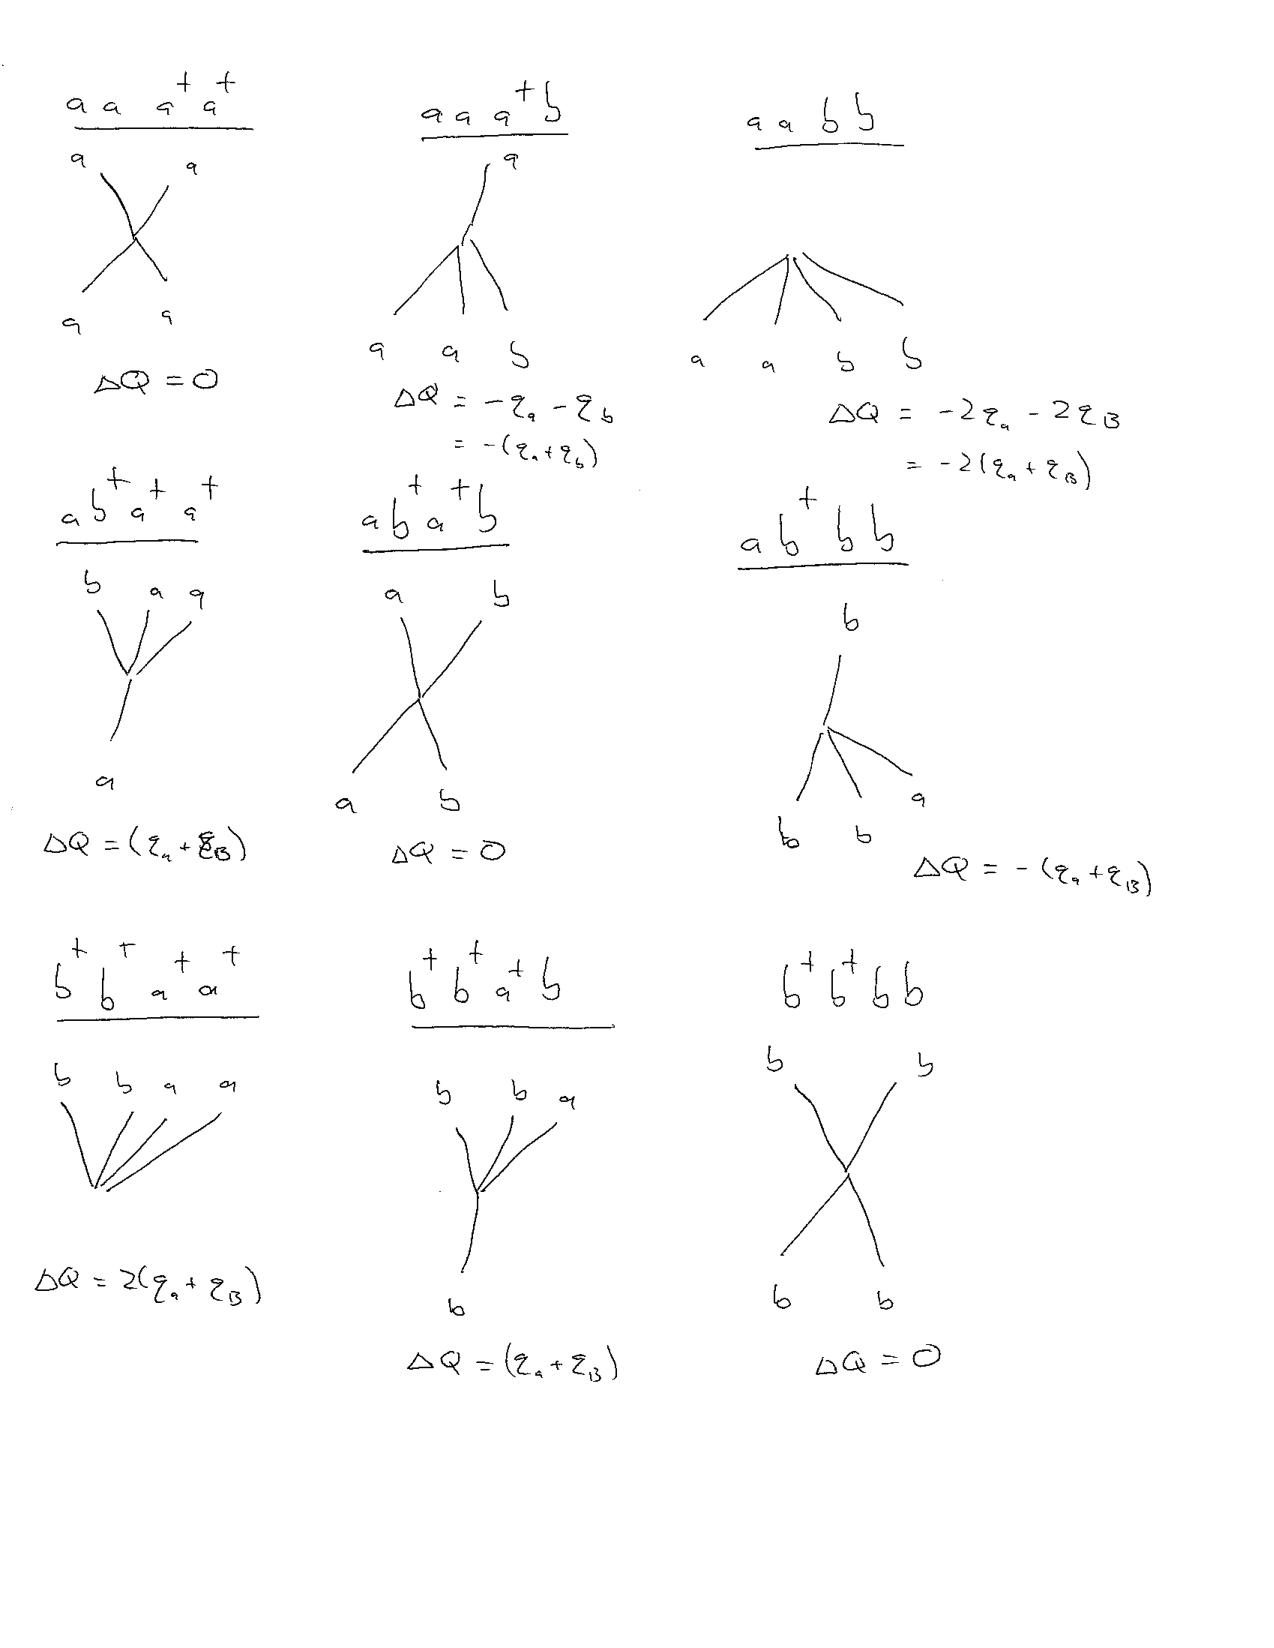
\includegraphics[width=0.9\textwidth]{./AntiParticlesSolutionb.pdf}
%\caption{A plot of the WIMP mass and interaction strength limits from the LUX experiment. From D. S. Akerib et al. [LUX Collaboration], “Results from a search for dark matter in the complete LUX exposure,” Phys. Rev. Lett. 118, no. 2, 021303 (2017) arXiv:1608.07648].}
\end{figure}

}
\item[c)] {Let the charge ($Q$) of particle $a$ be $q_a$ and the charge of particle $b$ be $q_b$.  Calculate $\Delta Q$ for each process.

See figure each term goes like $(q_a+q_b)$ 
 }
\item[d)] {What happens if you take $q_a = -q_b$ ?
When $q_a = -q_b$, all processes conserve charge.
}
\end{itemize}

%Sketch diagrams of the partile content of |psi(-inf)> to |psi(+inf)> for each term. like we did in class for a^\dagger a^\dagger a a = 

%LEt the charge of a be +q and the charge of b be -q, what is Delta(Q) in each of the interactions in b) ?



}

\end{document}
